\documentclass[11pt,english,compress]{beamer}
\usepackage[utf8]{inputenc}
\usepackage{verbatim}
\usepackage{eurosym}
\usepackage{ stmaryrd }
\usepackage{subfig}

\useoutertheme{smoothbars}
\useinnertheme[shadow=true]{rounded}
\usecolortheme{orchid}
\usecolortheme{whale}
\title{EzBench, a tool to help you benchmark and bisect the Graphics Stack's performance}
\subtitle{}
\author{Martin Peres}
\institute{Intel Open Source Technology Center Finland}

\AtBeginSection[]{
  \begin{frame}{Summary}
  \small \tableofcontents[currentsection, hideothersubsections]
  \end{frame} 
}
% 
% Tracking the performance of our complex graphics stack is a necessity to avoid unintentional regressions in the performance of the most important games and benchmarks. Such regressions lead to unhappy open source gaming enthusiasts and wasted developer time who need to track down performance regressions sometimes months after they got introduced. Fixing such performance issues may also be a challenge as the code that introduced them may have become a dependency for newer features.
% 
% The need for performance tracking is becoming more and more critical as the complexity of our open source drivers increases to reach a performance comparable to their closed-source equivalent. This increased complexity makes it more and more likely for commits to accidentally break the performance of some benchmark/games on some platforms that the developer may not have convenient access to.
% 
% In an effort to detect performance regressions before they even hit mainline, automation should be increased. However, when it can take up to an hour to test the performance of one commit on one benchmark, it becomes clear that we will never have the necessary hardware to be able to test all the commits found on the mailing lists and we will have to be smarter than this.
% 
% In this presentation, I will describe the different challenges found in benchmarking, some surprising results, some tricks to reduce the variance between runs and what is my current plan for improving our performance QA by automatically tracking the performance, bisecting performance changes and letting everyone know about them by auto answering on the mailing list.
% 
% Presenter: Martin Peres

\begin{document}

\setbeamertemplate{navigation symbols}{}

\begin{frame}
	\titlepage
\end{frame}

\section{Introduction}
\subsection*{Introduction}
\begin{frame}
	\frametitle{Introduction}

	\begin{block}{Current situation}
		\begin{itemize}
			\item Complex games/benchmarks are becoming available on Linux;
			\item Drivers are getting more complex as performance improves;
			\item Users now rely on Open Source drivers for performance.
		\end{itemize}
	\end{block}
	
	\pause
	
	\begin{block}{Risks when merging new code}
		\begin{itemize}
			\item Break previous functionalities / rendering;
			\item Break the performance of a game inadvertly;
			\item Improve the performance of one game but slow down others.
		\end{itemize}
	\end{block}
	
	\pause
	
	\begin{block}{}
		$\Rightarrow$ Need to benchmark all the platforms and games of interest.
	\end{block}
\end{frame}

\section{Benchmarking}
\subsection*{Who needs it?}
\begin{frame}
	\frametitle{Benchmarking}
	
	\begin{block}{Different needs for benchmarking}
		\begin{itemize}
			\item Developers: Run multiple experiments and compare them;
			\pause
			\item QA: Continuous Integration, performance bug reports.
		\end{itemize}
	\end{block}
\end{frame}

\subsection{Pitfalls}
\begin{frame}
	\frametitle{Pitfalls}
	
	\begin{block}{Pitfalls of benchmarking}
		\begin{itemize}
			\item Intra- and inter-runs variance depends on the benchmarks;\pause
			\item Hitting the power budget, a thermal limit or GPU reset;\pause
			\item Being able to reproduce the different test results;\pause
			\item Not using the expected libraries;
		\end{itemize}
	\end{block}
\end{frame}

\begin{frame}
	\frametitle{Example of variances}
	
	\begin{block}{}
		The variance forces us to execute multiple runs, which takes time!
	\end{block}
	
	\pause
	
	\begin{figure}%
		\centering
		\subfloat[Bad FPS distribution]{{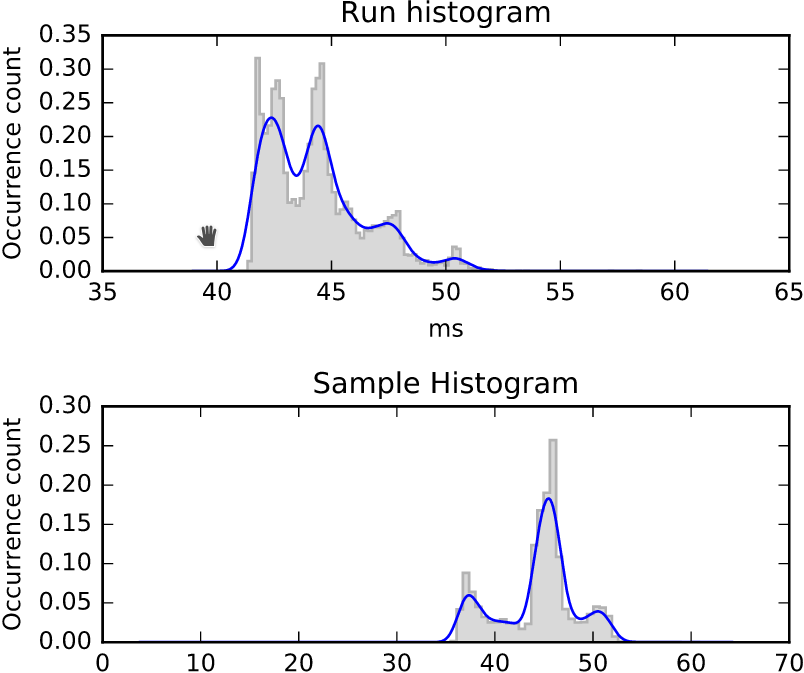
\includegraphics[width=5cm]{variance_bad.png} }}%
		\qquad
		\pause
		\subfloat[Good FPS distribution]{{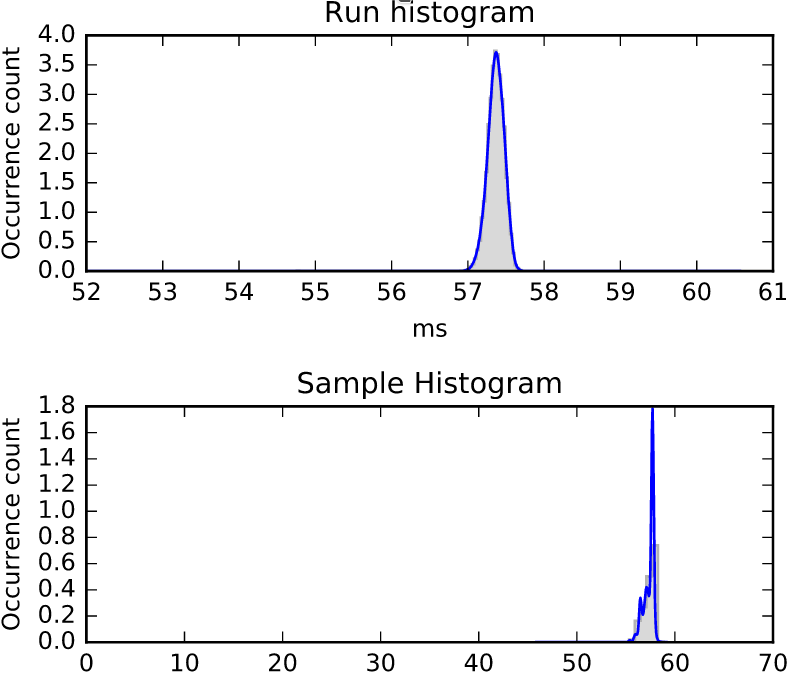
\includegraphics[width=5cm]{variance_good.png} }}%
		\caption{Examples of variance}%
	\end{figure}
\end{frame}

\subsection{Automating benchmarking}

\begin{frame}
	\frametitle{Automated benchmarking}

	\begin{block}{Objectives of automated benchmarking}
		\begin{itemize}
			\item Avoid or detect human errors;\pause
			\item Make sure the data is valid;\pause
			\item Be predictable in the execution time;\pause
			\item Provide as much information as possible;\pause
			\item Guarantee reproducibility of the results.
		\end{itemize}
	\end{block}
	
	\pause
	
	\begin{block}{In concrete goals}
		\begin{itemize}
			\item Be aware of every library used by the program;\pause
			\item Know their versions, git ID and compilation flags;\pause
			\item Poll on the resources' usage metrics; \pause
			\item Store all this information inside a report\pause;
			\item Understand performance results and act upon them.
		\end{itemize}
	\end{block}
\end{frame}

\begin{frame}
	\frametitle{Automated benchmarking - Making sure the data is valid}

	\begin{block}{Making sure the data is valid}
		\begin{itemize}
			\item Compute the statistical accuracy and add runs if needed;\pause
			\item Get information out from the kernel about major hw events;\pause
			\item Learn to give up and re-prioritise other benchmarks;\pause
			\item Try to reproduce runs and detect major differences;\pause
			\item Reboot the machine if unsure about the results;\pause
			\item Collect usage metrics of the resources;\pause
			\item Log all this information in the report.
		\end{itemize}
	\end{block}
	
	\pause
	
	\begin{block}{Bisect performance changes automatically}
		\begin{itemize}
			\item It adds credibility to the report;\pause
			\item It also reproduces the issue.
		\end{itemize}
	\end{block}
\end{frame}

\begin{frame}
	\frametitle{Automated benchmarking - Reading out the environment}

	\begin{block}{Listing dependencies}
		\begin{itemize}
			\item Using ldd is insufficient because of run-time dependencies;\pause
			\item Strace is the most robust approach but it is slow;\pause
			\item Linked libraries can be polled from /proc/\$pid/maps;\pause
			\item We can hook some functions using LD\_PRELOAD.
		\end{itemize}
	\end{block}
	
	\pause
	
	\begin{block}{Query the version of a library/program}
		\begin{itemize}
			\item No silver bullet;\pause
			\item Can sometimes be read out of a program (Linux);\pause
			\item Requires controlling the build process;\pause
			\item Requires package-kit for system libraries.
		\end{itemize}
	\end{block}
\end{frame}

\section{EzBench}
\subsection{Overview}
\begin{frame}
	\frametitle{EzBench - Overview}

	\begin{block}{Ezbench - Goals}
		\begin{itemize}
			\item Provide workflows and automation to take care of most issues;\pause
			\item Provide a framework quickly adaptable to your needs;\pause
			\item Work for both QA and developers!
		\end{itemize}
	\end{block}
	
	\pause
	
	\begin{block}{Authors}
		\begin{itemize}
			\item Authors: Martin Peres (Intel) \& Chris Wilson (Intel);
			\item Licence: MIT;
			\item Url: http://cgit.freedesktop.org/$\sim$mperes/ezbench/
		\end{itemize}
	\end{block}
\end{frame}

\subsection{Architecture and features}

\begin{frame}
	\frametitle{EzBench - Components}

	\begin{block}{Components}
		\begin{itemize}
			\item core.sh: simple runner;\pause
			\item env\_dump: dump environment;\pause
			\item ezbench: work scheduler;\pause
			\item utils/ezbench.py: framework;\pause
			\item utils/ezbenchd.py: work executer;\pause
			\item stats/compare\_reports.py: visualisation.
		\end{itemize}
	\end{block}
\end{frame}

\begin{frame}
	\frametitle{EzBench - SHA1-DB}

	\begin{block}{SHA1-DB}
		\begin{itemize}
			\item Stores SHA1 hashes of the libs you compile;\pause
			\item Allows you to attach metadata to the hash:\pause
			\begin{itemize}
				\item Git commit SHA1;\pause
				\item Compilation flags;\pause
				\item Whatever you want!
			\end{itemize}
		\end{itemize}
	\end{block}
\end{frame}

\begin{frame}
	\frametitle{EzBench - Env Dump}

	\begin{block}{Env Dump}
		\begin{itemize}
			\item Shared object LD\_PRELOADed when running benchmarks;\pause
			\item Captures information about:\pause
			\begin{itemize}
				\item HW topology (CPU, RAM, BIOS, MOTHERBOARD);\pause
				\item Dependencies to libraries, binaries and UNIX services;\pause
				\item X interactions (window/screen sizes);\pause
				\item GL/GLX/EGL contexts;\pause
				\item Environment variables.
			\end{itemize}
		\end{itemize}
	\end{block}
\end{frame}

\subsection{Demo}
\begin{frame}
	\frametitle{EzBench - Demo time!}

	\begin{block}{}
		Demo time and questions!
	\end{block}
\end{frame}

\subsection{Backup slides}
\begin{frame}
	\frametitle{EzBench - Features}

	\begin{block}{Current features}
		\begin{itemize}
			\item Modular architecture (profiles, tests and user hooks);\pause
			\item Automates the acquisition of benchmark data;\pause
			\item Generates a report that is usable by developers;\pause
			\item Bisects performance changes automatically;\pause
			\item Provides python bindings to acquire data and parse reports;\pause
			\item Be crash-resistant by storing the expected goal and comparing it to the current state;\pause
			\item Collect the environment information and diff it;\pause
			\item Detect the variance and peformance changes;\pause
			\item Automatically schedule more work to improve the report.
		\end{itemize}
	\end{block}
\end{frame}

\begin{frame}
	\frametitle{EzBench - Features}

	\begin{block}{TODO}
		\begin{itemize}
			\item Watchdog support;\pause
			\item Handle kernel boot failures;\pause
			\item Add support for PTS as a backend;\pause
			\item Better integrate the build process;\pause
			\item React to HW events such as throttling;\pause
			\item Reset the environment to a previous state;\pause
			\item Integrate with patchwork to test patch series;\pause
			\item Predict run times more accurately (compilation done);\pause
			\item Support sending emails to the authors of perf changes.
		\end{itemize}
	\end{block}
\end{frame}

\end{document}
